\documentclass[00-main.tex]{subfiles}
\begin{document}

\section*{Problem One}

\subsection*{a.}

\begin{minted}{matlab}
>> A = [2 1 0;1 4 3;2 4.5 6];
>> b = [2 0 -3.5]';
>> x = A\b
x =
   0.50000
   1.00000
  -1.50000
>> % Checking the answer:
>> A*x
ans =
   2.00000
   0.00000
  -3.50000
>> % Answer is b, as expected.
\end{minted}

\subsection*{b.}

\begin{minted}{matlab}
>> % Finding the LU-decomposition of A where L is the
>> % lower- and U is the upper triangular matrix.
>> [L U] = lu(A);
>> L
L =
   1.00000   0.00000   0.00000
   0.50000   1.00000   0.00000
   1.00000   1.00000   1.00000
>> U
U =
   2.00000   1.00000   0.00000
   0.00000   3.50000   3.00000
   0.00000   0.00000   3.00000
\end{minted}

\subsection*{c.}

\inputminted[linenos]{matlab}{newton_c.m}

\subsection*{d.}

\inputminted[linenos]{matlab}{newton_d.m}

\subsection*{e.}

\begin{minted}{matlab}
>> [t_1 y_1] = euler(@(t,y) -sin(y), 0, 10, 1.5, 0.1);
>> [t_2 y_2] = euler(@(t,y) y_1(floor(10*t+1)), 0, 10, 0, 0.1);
>> plot(t_1, y_1, t_2, y_2);
\end{minted}

\begin{figure}
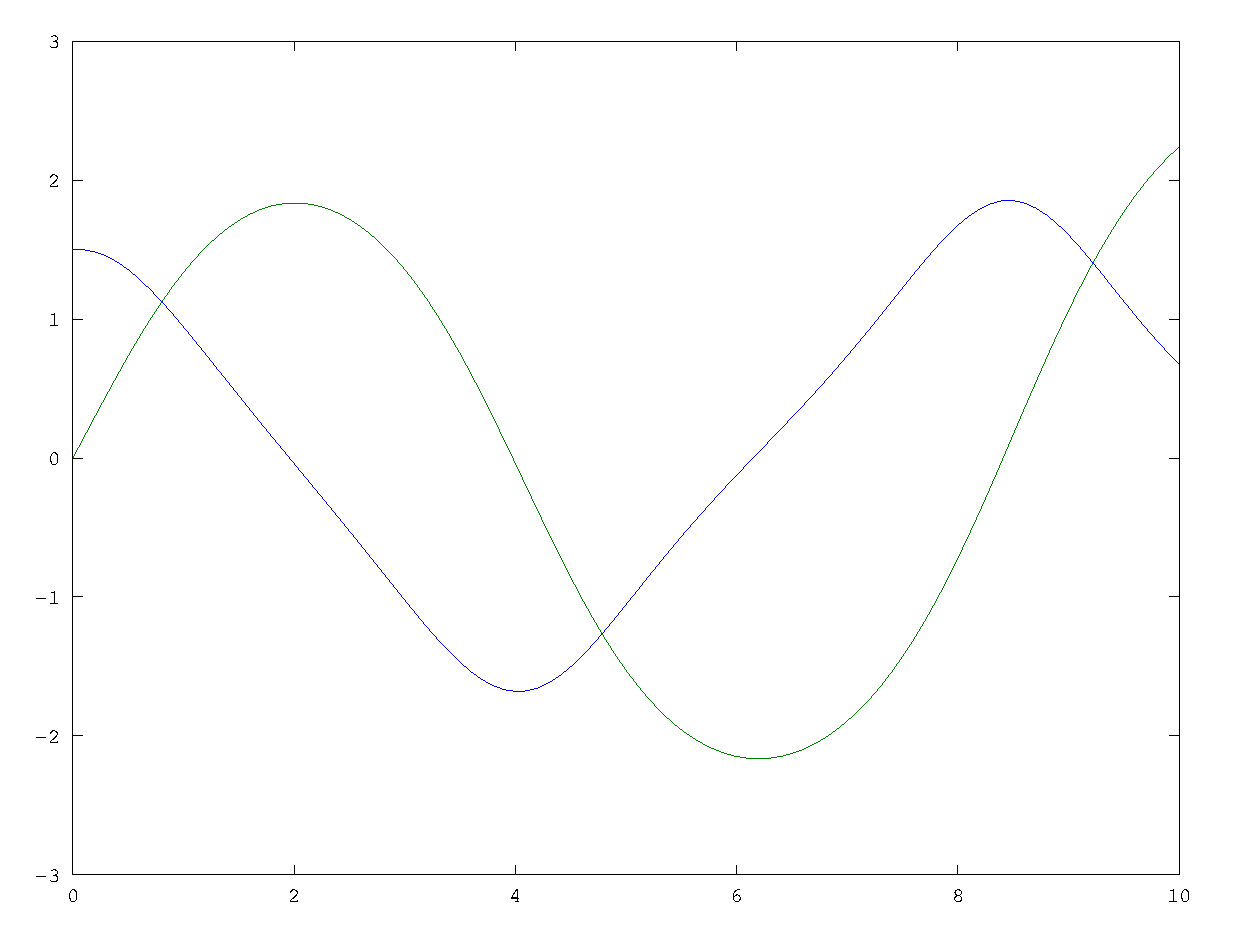
\includegraphics[width=\textwidth]{euler_plot}
\caption{Plot shows $y_1$ and $y_2$ that was found through Euler's method.}
\end{figure}


%\bibliosub
\end{document}